 
\documentclass[a4paper,titlepaget]{article}
\usepackage[T1]{fontenc}
\usepackage[utf8]{inputenc}
\usepackage[english]{babel}
\usepackage{amsmath}
\usepackage{graphicx}
\usepackage{graphics}
\usepackage{caption}
\usepackage{amssymb}
\usepackage{listings}
\textwidth=450pt\oddsidemargin=0pt
\date{15 May 2020}



\begin{document}
	\begin{titlepage}
		\begin{center}
			
\includegraphics[width=1.8cm, height=1.8cm]{Images/logounipd}\qquad\qquad{{\Large{\textsc{Universit\`a degli Studi di Padova}}}}\qquad\qquad
\includegraphics[width=2.8cm, height=1.9cm]{images/logodei}
		\end{center}
		\begin{center}
            \rule[0.1cm]{15.8cm}{0.1mm}
			\rule[0.5cm]{15.8cm}{0.6mm}
			{\small{\bf Master Degree Course in Computer Engineering}}
			
		\end{center}
		\vspace{40mm}
		\begin{center}
			{\LARGE{\bf Homework 4}}
			
			\vspace{7mm}
			
			{\Large{\bf Report of the laboratory 6: Object Recognition and Tracking}}
			
			\vspace{15mm} 
			{\large{Course of Computer Vision, second semester 2019/2020}}
			\vspace{19mm} 
		\end{center}
		\vspace{10mm}
		\par
		\vspace{40mm}
			\begin{minipage}{0.5\textwidth}
				{\large{\bf Alex De Toffol (1207658)\\}}
				\newline
				{\large{\bf Luca Dolci (1234008)\\}}
			\end{minipage}%
			\begin{minipage}{0.5\textwidth}
			\end{minipage}%
	\end{titlepage}

\newpage

\section{Introduction}
In this laboratory an input video is taken from the command line, showing four books placed on a table to which translations and rotations are performed.
The video is processed as follows:
\begin{itemize}
	\item The first frame is extracted from the file and the strongest local features are localized. Four images, corresponding to the four principal objects in the video, are used as a reference; thanks to these operations, it is possible to draw the rectangular outline of each book.
	\item Subsequently, the following frames are analyzed and the movement of each book is tracked using the Lucas Kanade Feature Tracker. Each rectangle is moved together with its corresponding book.	
\end{itemize}
In order to run the program, build it with cmake and inside the build folder type:
\begin{lstlisting}[language=bash]
	$ ./lab6 video_path objects_folder_path objects_extension
\end{lstlisting}
You can set various parameters. Check the help for that (execute with -h)

\newpage

\section{Object Recognition}
The inputs of this task are two:
\begin{itemize}
	\item The first frame of the video which is obtained decomposing the video into single frames and selecting the first one. This frame shows 4 books placed on a table.
	\item A set of reference objects, which is given ready to use and it is composed by one image for each object representing the frontal cover of the book. In order to increase performances, the set of objects has been processed to remove the unnecessary edges and to better identify the relevant parts.
\end{itemize}

\begin{figure}[!htb]
	\centering
	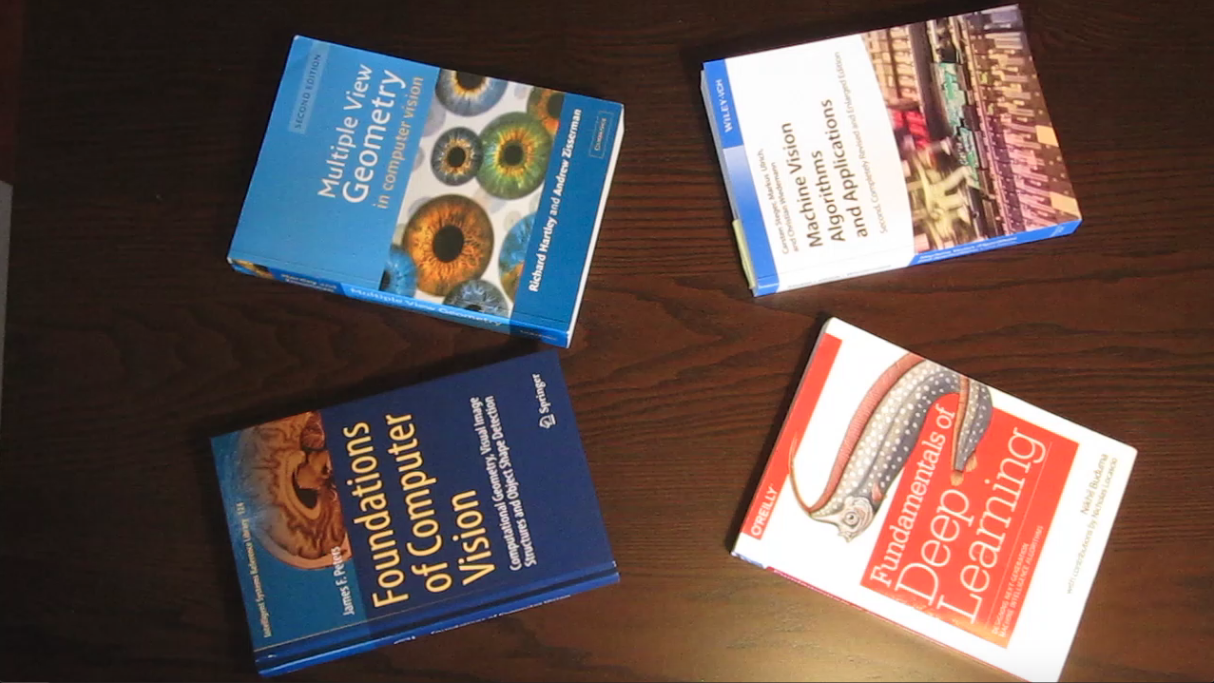
\includegraphics[width=.8\textwidth]{images/first-frame}
	\caption{The first frame of the video}
\end{figure}

\begin{figure}[htpb] 
\begin{minipage}{.2\textwidth}

\includegraphics[width=\textwidth, height=0.2\textheight]{images/obj1} 
\end{minipage}
\hspace{.05\textwidth}
\begin{minipage}{.2\textwidth}

\includegraphics[width=\textwidth, height=0.2\textheight]{images/obj2}
\end{minipage}  
\hspace{.05\textwidth}
\begin{minipage}{.2\textwidth}  
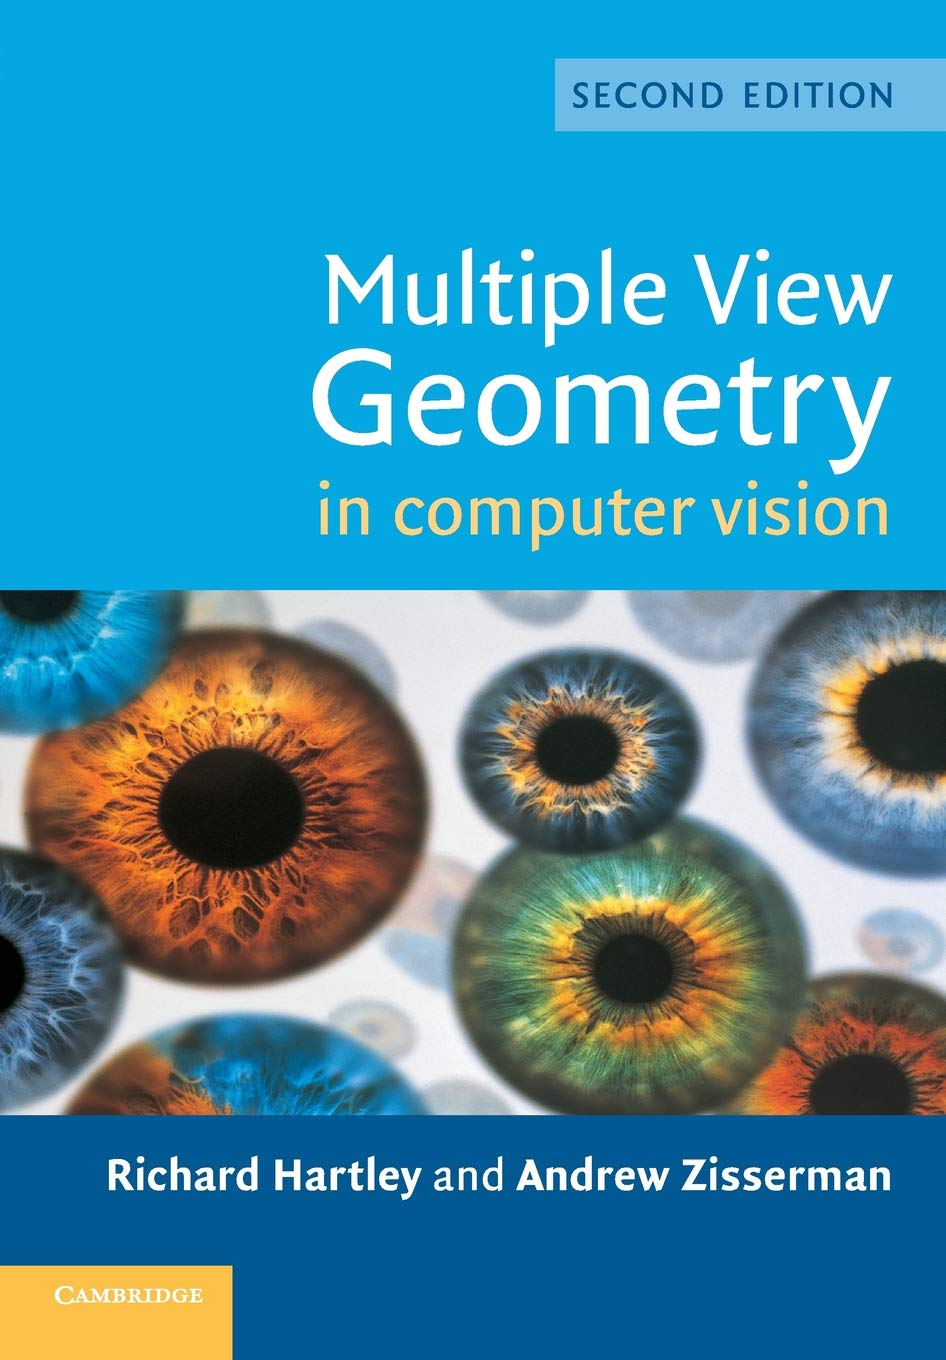
\includegraphics[width=\textwidth, height=0.2\textheight]{images/obj3}
\end{minipage} 
\hspace{.05\textwidth}
\begin{minipage}{.2\textwidth}  
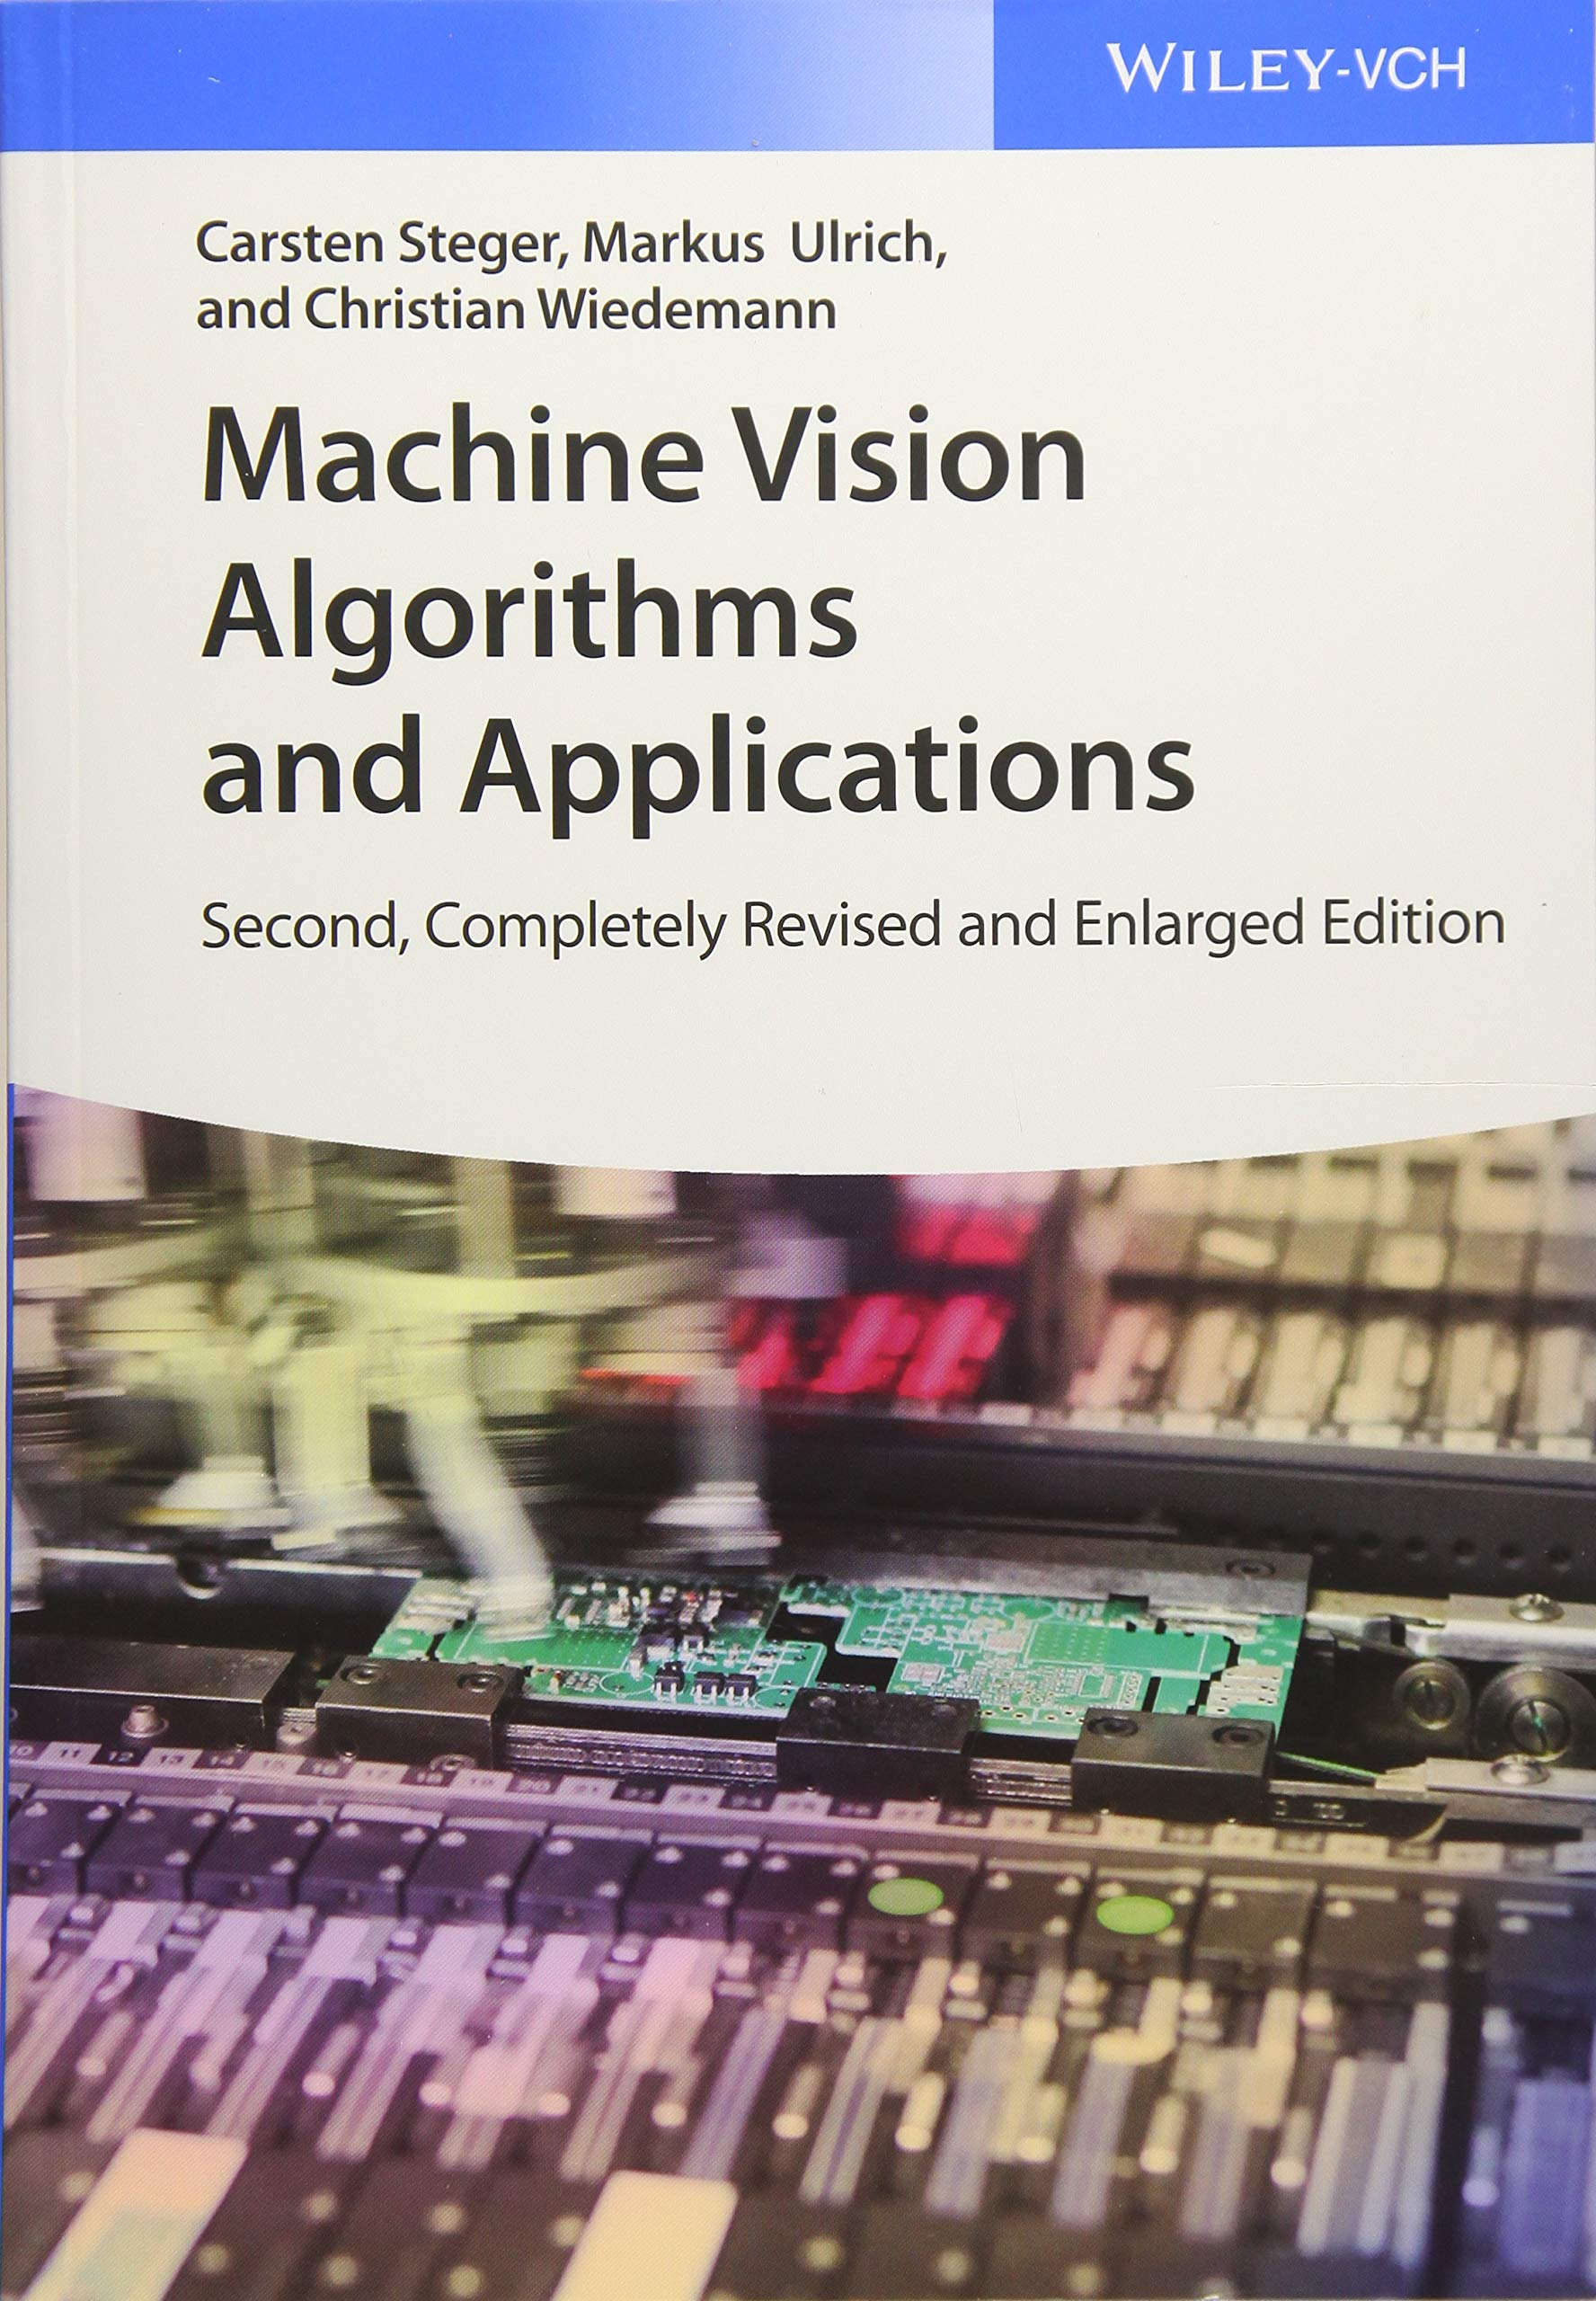
\includegraphics[width=\textwidth, height=0.2\textheight]{images/obj4}
\end{minipage} 
\caption{The set of reference objects}
\end{figure}

The \texttt{matchFirstFrame} method is implemented; for each different reference object, the keypoints and the descriptors are extracted using the SIFT algorithm and the matches between the first frame and the reference object are computed.
The matches with distance greater than 3 times the minimum distance among all the matches are dropped and not considered to improve the quality of the results. 
The ratio is set to 3 and it gives good resuts but slightly different values work good as well (ratio values that make the program crash are managed in order to avoid this unwanted event).

Moreover, the RANSAC algorithm is used to improve the set of matches and to be strong against outliers.
Eventually, a rectangle around each cover is drawn with a different color.

\begin{figure}[htpb]
	\centering
	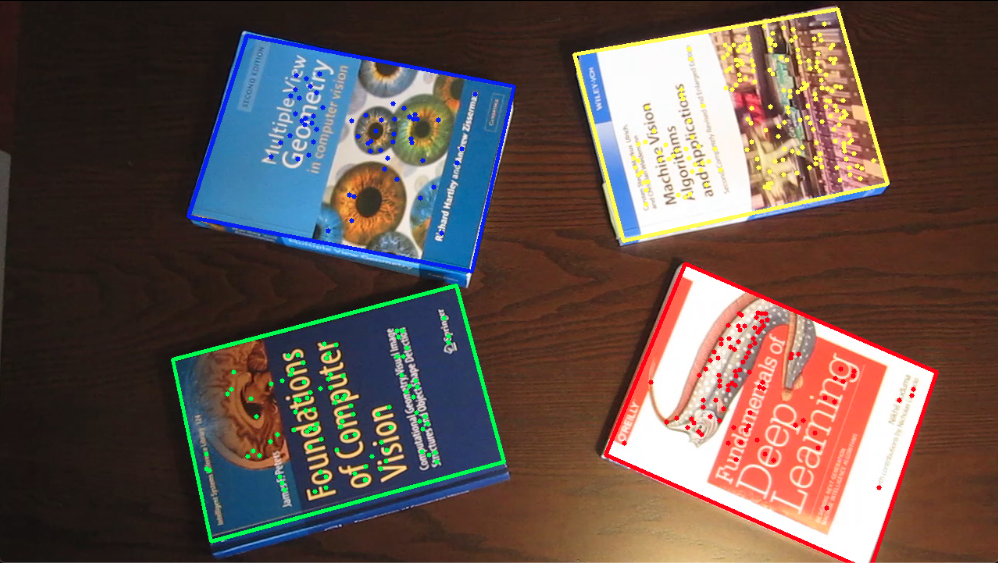
\includegraphics[width=.8\textwidth]{images/keypoints-rectangles}
	\caption{The computed keypoints and the rectangles corresponding to each cover}
\end{figure}

\newpage

\section{Tracking}
Once we have the first set of matched features, one for each object, it is possible to track their positions in the next frames. This is done by \emph{Optical Flow} and, in particular, using \emph{Lucas Kanade's algorithm}, since we want to track sparse feature sets. 

In the OpenCV library, the algorithm is implemented in
the \texttt{calcOpticalFlowPyrLK} function which takes as input:
\begin{itemize}
	\item The previous frame, the one with all the points in the right place
	\item The position of these keypoints
	\item The next frame, the target one
	\item The size of the search window
	\item Other values that are left unchanged at their default value 
\end{itemize}
One parameter to which particular attention is paid is the size of the window; it is set to 31x31 pixels because it works well for the video provided.
In fact, using a smaller one, the tracking of the features is not correct since it breaks the space coeherence assumption, a foundation of LK algorithm. 
However, values greater than 15x15 provide decent results in terms of accuracy but very high value makes the computational power requested infeasible. 
This is the reason why 31x31 is selected as a good trade-off. 
It is also possible to skip some frames (up to three) reducing the computational power requested for the whole video computations without big losses of accuracy.

The next step is to eliminate outliers. 
This can be done using two additional returns from the previous function:
\begin{itemize}
	\item Status variable: when the algorithm is not capable to detect the position of a feature in the new frame, the feature is eliminated.
	\item Error variable: since the \emph{flags} parameter of the function is left as default, the error measure for each feature is computed as the $l_1$ distance between the keypoint in the new and previous frame divided by the window size. Features with high errors (greater than some standard deviation from the mean of errors) are eliminated.
 \end{itemize}
If the number of remaining features is low, fewer features are eliminated. This can be seen as a regularization mechanism against high values of ratio: after this step, the number of features remains stable (around 150/200 for each object).

The last step is to compute the Homography matrix in order to draw all the
rectangles.

\begin{figure}[htpb]
	\centering
	\captionsetup{justification=centering}
	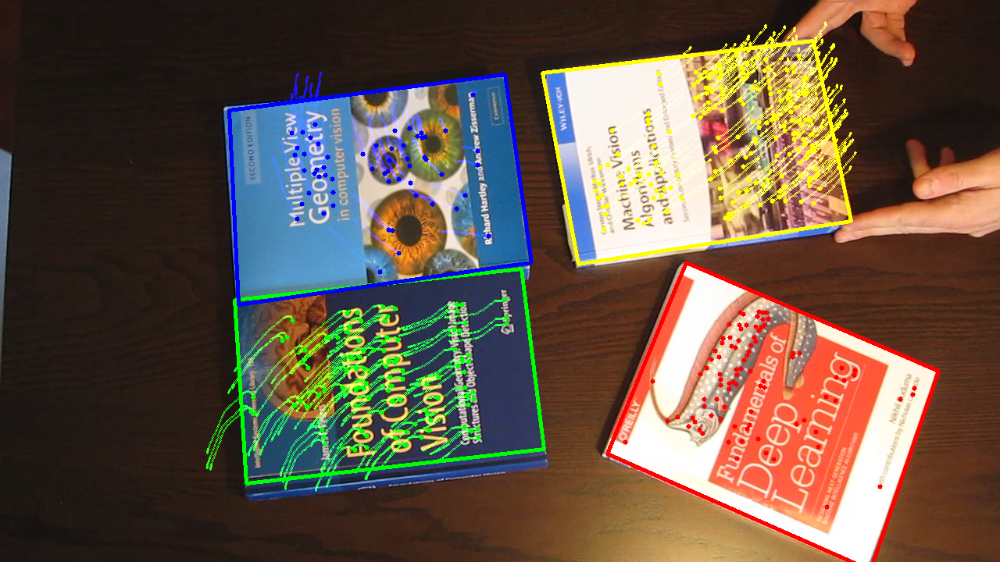
\includegraphics[width=.7\textwidth]{images/tracking_keypoints}
    \caption{Keypoints tracked during book's movement. (Execute with
    -draw$\_$keypoints=1 and -draw$\_$tracking=1 to be able to see the effect)}
\end{figure}
\begin{figure}[htpb]
	\centering
	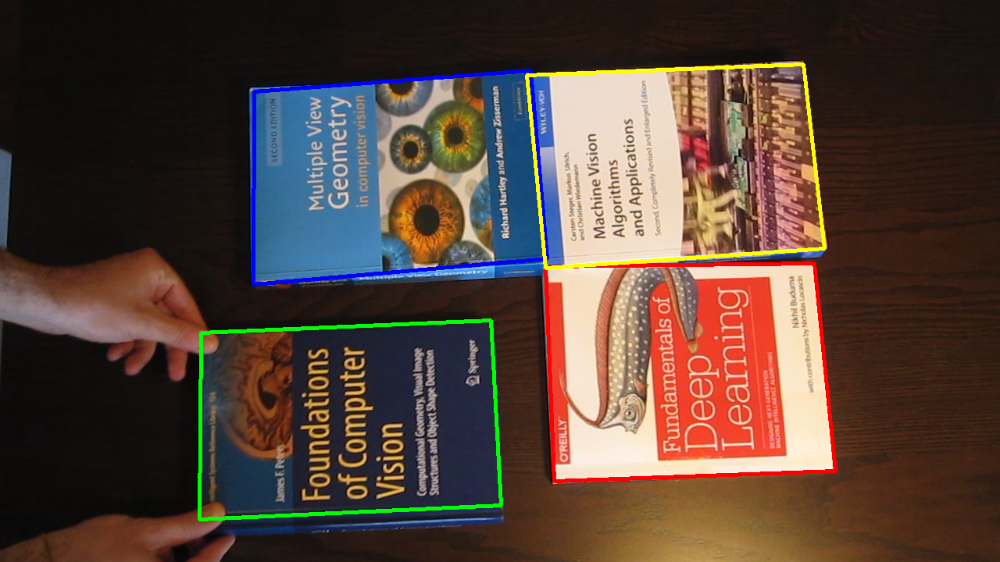
\includegraphics[width=.7\textwidth]{images/tracking_rectangles}
    \caption{An example of drawn rectangles during tracking}
\end{figure}

\end{document}l
